\subsection{Section 2.2}
\begin{tcolorbox}[
        title={Problem 8 (a)},
        valign=center,
        nobeforeafter,
        colframe=gray!95!black
    ]
Compute the following limit if it exists:
    \begin{align}
        \lim_{(x, y) \rightarrow (0, 0)} \frac{(x + y)^2 - (x - y)^2}{xy}
    \end{align}
\end{tcolorbox}

\begin{claim}
    The limit exists and is given by:
    \begin{align}
        \lim_{(x, y) \rightarrow (0, 0)} \frac{(x + y)^2 - (x - y)^2}{xy} &= 4
    \end{align}
\end{claim}

\begin{proof} We proceed by direct computation:
    \begin{align*}
        \lim_{(x, y) \rightarrow (0, 0)} \frac{(x + y)^2 - (x - y)^2}{xy} &= \lim_{(x, y) \rightarrow (0, 0)} \frac{\left(x^2 + 2xy + y^2\right) - \left(x^2 - 2xy + y^2\right)}{xy} \\
        &= \lim_{(x, y) \rightarrow (0, 0)} \frac{4xy}{xy} \\
        &= \lim_{(x, y) \rightarrow (0, 0)} 4 \\
        &= 4
    \end{align*}
\end{proof}

\begin{tcolorbox}[
        title={Problem 8 (b)},
        valign=center,
        nobeforeafter,
        colframe=gray!95!black
    ]
Compute the following limit if it exists:
    \begin{align}
        \lim_{(x, y) \rightarrow (0, 0)} \frac{\sin(xy)}{y}
    \end{align}
\end{tcolorbox}

\begin{claim}
    The limit exists and is given by:
    \begin{align}
        \lim_{(x, y) \rightarrow (0, 0)} \frac{\sin(xy)}{y} &= 0
    \end{align}
\end{claim}

\begin{proof}
\textit{(Taylor expansion)}

Observe that \(xy\) is small since \((x, y) \rightarrow (0, 0)\). 

Consider:
    \begin{align}
        \sin(t) &= t - \frac{t^3}{3!} + \frac{t^5}{5!} + ...
    \end{align}

\newpage 

Let \(t = xy\). This approximation is valid since \(xy\) is small Then:
    \begin{align*}
        \lim_{(x, y) \rightarrow (0, 0)} \frac{\sin(xy)}{y} &\approx \lim_{(x, y) \rightarrow (0, 0)} \frac{\left(xy - \frac{(xy)^3}{3!} + \frac{(xy)^5}{5!} + ...\right)}{y} \\
        &= \lim_{(x, y) \rightarrow (0, 0)} \frac{xy}{y} - \frac{(xy)^3}{3!y} + \frac{(xy)^5}{5!y} + ... \\
        &= \lim_{(x, y) \rightarrow (0, 0)} x - \frac{x^3y^2}{3!} + \frac{x^5y^4}{5!} + ... \\
        &= 0
    \end{align*}
\end{proof}

\begin{proof}
\textit{(\(\operatorname{sinc}\) function)}

Observe that \(xy\) is small since \((x, y) \rightarrow (0, 0)\). 

Recall from single variable calculus, proven by the Squeeze Theorem:
    \begin{align}
        \lim_{t \rightarrow 0} \frac{\sin(t)}{t} &= 1
    \end{align}

Let \(t = xy\). This approximation is valid since \(xy\) is small.

Then:
    \begin{align*}
        \lim_{(x, y) \rightarrow (0, 0)} \frac{\sin(xy)}{y} &= \lim_{(x, y) \rightarrow (0, 0)} x\frac{\sin(xy)}{xy} \\
        &= \lim_{(x, y) \rightarrow (0, 0)} x \cdot \lim_{(x, y) \rightarrow (0, 0)} \frac{\sin(xy)}{xy} \\
        &= 0 \cdot 1 \\
        &= 0
    \end{align*}
\end{proof}

\begin{tcolorbox}[
        title={Problem 26},
        valign=center,
        nobeforeafter,
        colframe=gray!95!black
    ]
Using either the \(\varepsilon - \delta\) definition of the limit or spherical coordinates, show that: 
    \begin{align}
        \lim_{(x, y, z) \rightarrow (0, 0, 0)} \frac{xyz}{x^2 + y^2 + z^2} &= 0
    \end{align}
\end{tcolorbox}

\begin{proof}
\textit{(\(\varepsilon - \delta\) definition)} 

Recall the \(\varepsilon - \delta\) definition of the limit. 

We say that \(\displaystyle \lim_{\vec{x} \rightarrow \vec{x}_0} f(\vec{x}) = L\) if for every \(\varepsilon > 0\), there exists a \(\delta > 0\) such that for all \((x, y, z)\):
\begin{align}
    \|\vec{x} - \vec{x}_0\| < \delta &\implies |f(\vec{x}) - L| < \varepsilon
\end{align}

In this problem, \(\vec{x}_0 = 0\) and \(L = 0\). We must show that for every \(\varepsilon > 0\), there exists a \(\delta > 0\) such that for all \((x, y, z)\):
\begin{align}
    \|\vec{x}\| < \delta &\implies |f(\vec{x}) - 0| < \varepsilon
\end{align}

Observe that, for all \(x\), \(y\), \(z \in \mathbb{R}\):
\begin{align}
    \left|\frac{x}{\sqrt{x^2 + y^2 + z^2}}\right| &\leq 1
\end{align}

Consider \(\delta = \varepsilon\):
\begin{align*}
    \left|\frac{xyz}{x^2 + y^2 + z^2} - 0\right| &= \left|\frac{xyz}{x^2 + y^2 + z^2}\right| \\
    &= \left|\frac{xyz}{x^2 + y^2 + z^2}\frac{\sqrt{x^2 + y^2 + z^2}}{\sqrt{x^2 + y^2 + z^2}}\right| \\
    &= \left|\frac{x}{\sqrt{x^2 + y^2 + z^2}}\frac{y}{\sqrt{x^2 + y^2 + z^2}}\frac{z}{\sqrt{x^2 + y^2 + z^2}}\sqrt{x^2 + y^2 + z^2}\right| \\
    &= \left|\frac{x}{\sqrt{x^2 + y^2 + z^2}}\right|\left|\frac{y}{\sqrt{x^2 + y^2 + z^2}}\right|\left|\frac{z}{\sqrt{x^2 + y^2 + z^2}}\right|\left|\sqrt{x^2 + y^2 + z^2}\right| \\
    &\leq 1 \cdot 1 \cdot 1 \cdot \left|\sqrt{x^2 + y^2 + z^2}\right| \\
    &= \left|\sqrt{x^2 + y^2 + z^2}\right| \\
    &= \|\vec{x}\| \\
    &< \delta \\
    &= \varepsilon
\end{align*}
\end{proof}

\begin{proof}
\textit{(Spherical coordinates)} 

Recall spherical coordinates:
\begin{align}
    x &= \rho \cos(\theta) \sin(\varphi) & y &= \rho \sin(\theta) \sin(\varphi) & z &= \rho \cos(\varphi) & \rho &= \sqrt{x^2 + y^2 + z^2}
\end{align}

Observe that, regardless of angle:
\begin{align}
    |\cos{(\theta)}| &\leq 1 & |\sin{(\theta)}| &\leq 1
\end{align}

Then:
\begin{align*}
    \left|\frac{xyz}{x^2 + y^2 + z^2}\right| &= \left|\frac{\rho \cos(\theta) \sin(\varphi)\rho \sin(\theta) \sin(\varphi)\rho \cos(\varphi)}{\rho^2}\right| \\
    &= \left|\rho \cos(\theta) \sin(\theta) \cos(\varphi) \sin^2(\varphi)\right| \\
    &= \left|\rho\right| \left|\cos(\theta)\right| \left|\sin(\theta)\right| \left|\cos(\varphi)\right| \left|\sin(\varphi)\right|^2 \\
    &\leq \left|\rho\right| 
\end{align*}

Since taking the limit as \((x, y, z) \rightarrow (0, 0, 0)\) is equivalent to shrinking the norm of the vector \((x, y, z)\) to zero, in spherical coordinates we will only be concerned with taking the limit as \(\rho \rightarrow 0\):
    \begin{align*}
        \lim_{(x, y, z) \rightarrow (0, 0, 0)} \left|\frac{xyz}{x^2 + y^2 + z^2}\right| &\leq \lim_{\rho \rightarrow 0} |\rho| \\
        &= 0
    \end{align*}
    
Therefore, by the Squeeze Theorem:
\begin{align}
        \lim_{(x, y, z) \rightarrow (0, 0, 0)} \frac{xyz}{x^2 + y^2 + z^2} &= 0
    \end{align}
\end{proof}

\subsection{Section 2.6}

\begin{tcolorbox}[
        title={Problem 16},
        valign=center,
        nobeforeafter,
        colframe=gray!95!black
    ]
Let \(f(x, y) = -\sqrt{1 - x^2 - y^2}\) for \((x, y)\) such that \(x^2 + y^2 < 1\). \\

Show that the plane tangent to the graph of \(f\) at \((x_0, y_0, f(x_0, y_0))\) is orthogonal to the vector with components \((x_0, y_0, f(x_0, y_0))\). Interpret this geometrically.
\end{tcolorbox}

\begin{proof}
    We first compute the partial derivatives of \(f\):
    \begin{align*}
        \frac{\partial f(x_0, y_0)}{\partial x} &= \frac{x}{\sqrt{1 - x^2 - y^2}}\Biggr|_{(x, y) = (x_0, y_0)} & \frac{\partial f(x_0, y_0)}{\partial y} &= \frac{y}{\sqrt{1 - x^2 - y^2}}\Biggr|_{(x, y) = (x_0, y_0)} \\
        &= \frac{x_0}{\sqrt{1 - x_0^2 - y_0^2}} & &= \frac{y_0}{\sqrt{1 - x_0^2 - y_0^2}}
    \end{align*}
    
    The equation of the plane tangent to the graph of \(f\) at \((x_0, y_0, f(x_0, y_0))\) is given by:
    \begin{align}
        z - f(x_0, y_0) &= \frac{\partial f(x_0, y_0)}{\partial x}(x - x_0) + \frac{\partial f(x_0, y_0)}{\partial y}(y - y_0)
    \end{align}
    
    The normal vector of this tangent plane is given by:
    \begin{align}
        \vec{n} &= \left(\frac{\partial f(x_0, y_0)}{\partial x}, \frac{\partial f(x_0, y_0)}{\partial y}, -1\right) \\
        &= \left(\frac{x_0}{\sqrt{1 - x_0^2 - y_0^2}}, \frac{y_0}{\sqrt{1 - x_0^2 - y_0^2}}, -1\right) 
    \end{align}
    
    In order to show that the plane tangent to the graph of \(f\) at \((x_0, y_0, f(x_0, y_0))\) is orthogonal to the vector with components \((x_0, y_0, f(x_0, y_0))\), it is sufficient to show that the normal vector of the tangent plane is parallel to the vector with components \((x_0, y_0, f(x_0, y_0))\).
    
    Equivalently, we want to show that there exists some constant \(k\) such that:
    \begin{align}
        k \vec{n} &= (x_0, y_0, f(x_0, y_0)) \\
        k \left(\frac{x_0}{\sqrt{1 - x_0^2 - y_0^2}}, \frac{y_0}{\sqrt{1 - x_0^2 - y_0^2}}, -1\right) &= \left(x_0, y_0, -\sqrt{1 - x_0^2 - y_0^2}\right) \\
        \left(\frac{kx_0}{\sqrt{1 - x_0^2 - y_0^2}}, \frac{ky_0}{\sqrt{1 - x_0^2 - y_0^2}}, -k\right) &= \left(x_0, y_0, -\sqrt{1 - x_0^2 - y_0^2}\right)
    \end{align}
    
    Then:
    \begin{align*}
        \begin{cases}
            \frac{kx_0}{\sqrt{1 - x_0^2 - y_0^2}} &= x_0 \\
            \frac{ky_0}{\sqrt{1 - x_0^2 - y_0^2}} &= y_0 \\
            -k &= -\sqrt{1 - x_0^2 - y_0^2}
        \end{cases} 
        &= 
        \begin{cases}
            kx_0 &= x_0 \sqrt{1 - x_0^2 - y_0^2} \\
            ky_0 &= y_0 \sqrt{1 - x_0^2 - y_0^2} \\
            k &= \sqrt{1 - x_0^2 - y_0^2}
        \end{cases} \\
        &= 
        \begin{cases}
            k &= \sqrt{1 - x_0^2 - y_0^2} \\
            k &= \sqrt{1 - x_0^2 - y_0^2} \\
            k &= \sqrt{1 - x_0^2 - y_0^2}
        \end{cases}
    \end{align*}
    
    Therefore, the plane tangent to the graph of \(f\) at \((x_0, y_0, f(x_0, y_0))\) is orthogonal to the vector with components \((x_0, y_0, f(x_0, y_0))\).
\end{proof}

\textit{Geometric interpretation.} Let \(f(x, y) = z\).

Observe that \(f\) is geometrically the southern hemisphere of the unit sphere:
\begin{align*}
    z &= -\sqrt{1 - x^2 - y^2} \\
    z^2 &= 1 - x^2 - y^2 \\
    x^2 + y^2 + z^2 &= 1
\end{align*}

Observe also that \((x_0, y_0, f(x_0, y_0)) = (x_0, y_0, z_0)\) is the position vector at the point \((x_0, y_0, z_0)\) on the sphere.

This implies that the plane tangent to any point on the southern hemisphere of the unit sphere is orthogonal to the position vector at that point. More generally, this is true for all spheres centered at the origin.

\begin{figure}[h!]
    \centering
    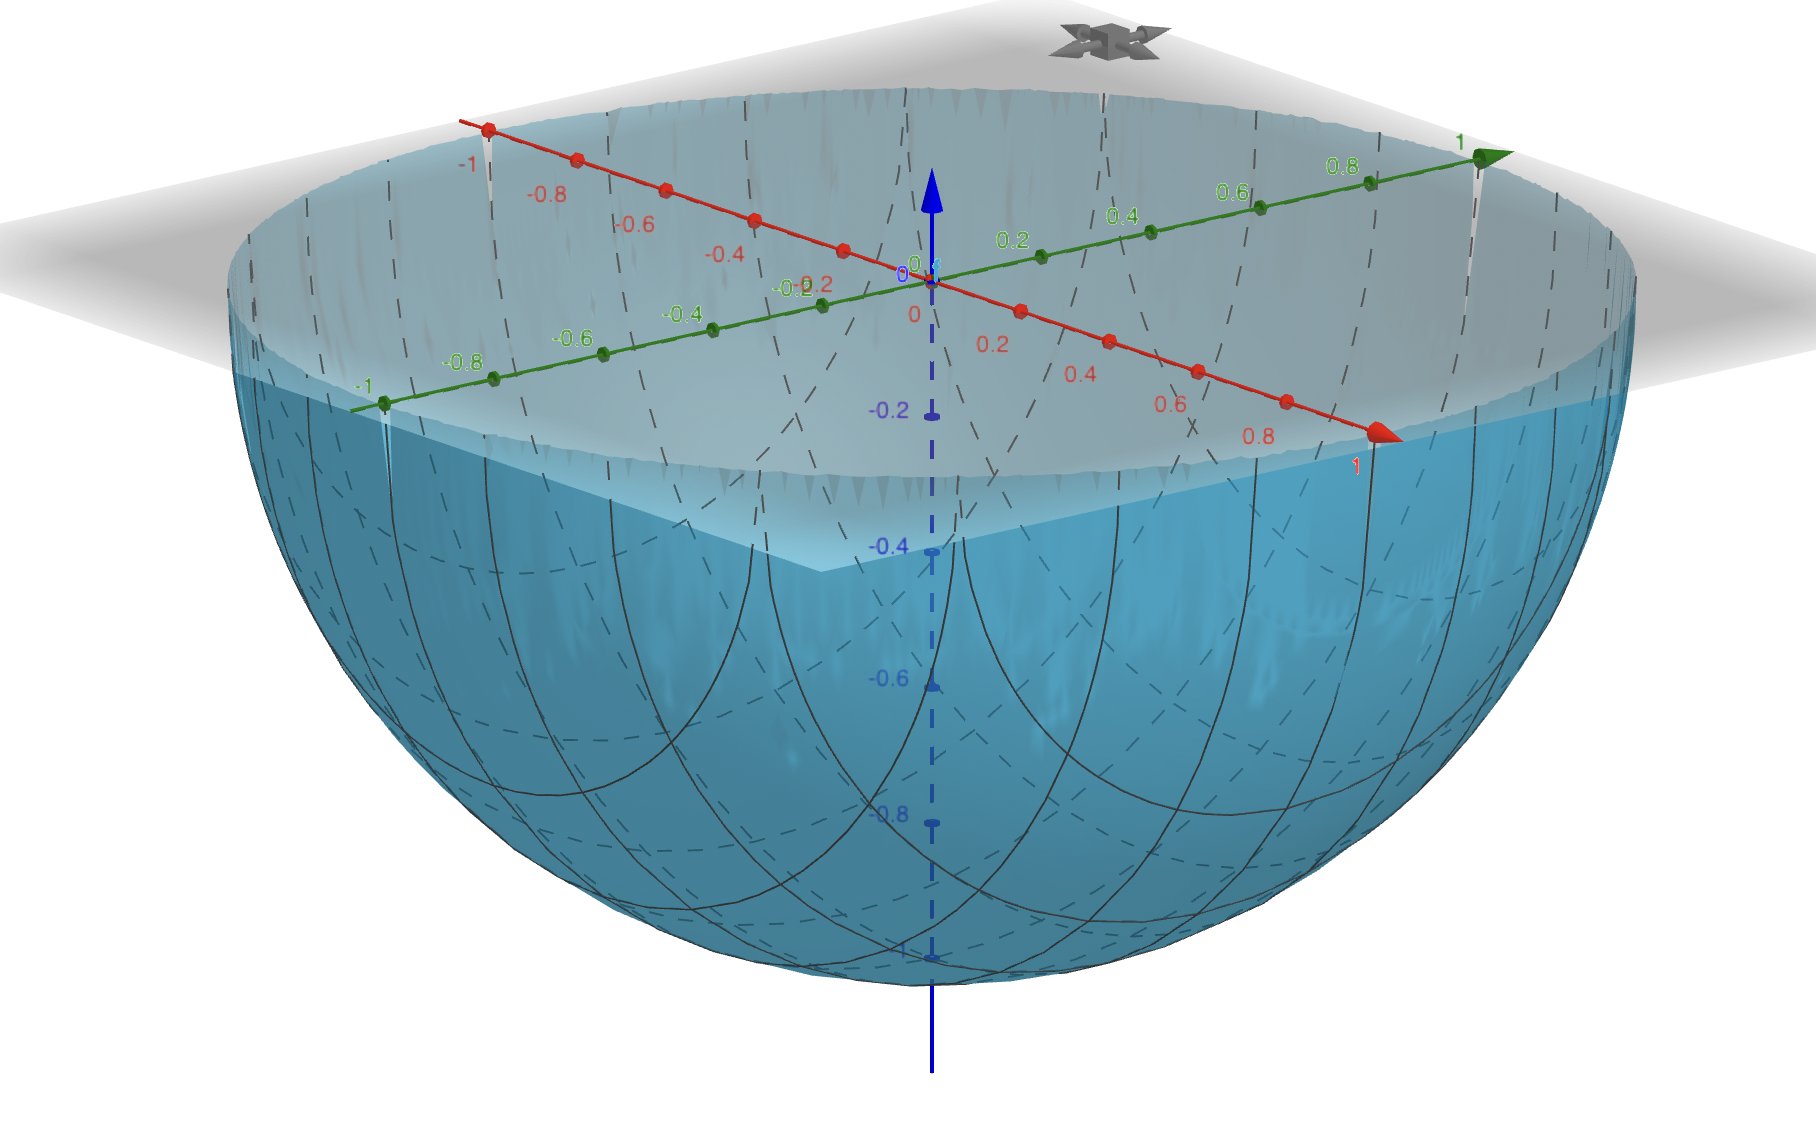
\includegraphics[width=15cm]{Pictures/Tutorial 1-1.png}
    \caption{Graph of \(f(x, y) = -\sqrt{1 - x^2 - y^2}\), which is the lower hemisphere of the unit sphere. Any position vector on the surface \((x,y,f(x,y))\) is normal to the surface.}
\end{figure}